\documentclass[a4paper, 11pt]{scrartcl}
\usepackage[margin=2.5cm
%,showframe%
]{geometry}
\usepackage[utf8]{inputenc}
\usepackage{fouriernc}
\usepackage[english]{babel}
\usepackage{fancyhdr}
\usepackage{graphicx}
\usepackage{subcaption}
\usepackage{bm}
\usepackage{amsmath}
%\usepackage{amsfonts}
%\usepackage{amssymb}
\usepackage{trfsigns}
\usepackage{xcolor}

%matplotlib colors:
%https://matplotlib.org/stable/tutorials/colors/colors.html
\definecolor{C0}{HTML}{1f77b4}
\definecolor{C1}{HTML}{ff7f0e}
\definecolor{C2}{HTML}{2ca02c}
\definecolor{C3}{HTML}{d62728}
\definecolor{C4}{HTML}{9467bd}
\definecolor{C5}{HTML}{8c564b}
\definecolor{C6}{HTML}{e377c2}
\definecolor{C7}{HTML}{7f7f7f}
\definecolor{C8}{HTML}{bcbd22}
\definecolor{C9}{HTML}{17becf}

\begin{document}
\pagestyle{fancy}
\fancyhf{} % clr
\fancyhead[L]{Data-Driven Methods in Signal Processing (Module \#24512)}
\fancyhead[R]{Tutorial: Matrix Fundamentals}
\fancyfoot[L]{frank.schultz@uni-rostock.de, INT, IEF}
\fancyfoot[C]{\thepage}
\fancyfoot[R]{WS 2026/27}

\section{Reduced Row Echelon Form of a Matrix}
\label{sec:rref}
The matrix $\bm{A}$ and its reduced row echelon form $\bm{R}_0$ obtained by Gauss-Jordan elimination
$$
\bm{A} =
\begin{bmatrix}
2 & \sqrt{5} & 0\\
0 & 0 & 1\\
0 & 0 & 0\\
0 & 0 & 0
\end{bmatrix}
\quad\rightarrow\quad
\bm{R}_0 =
\begin{bmatrix}
1 & \frac{\sqrt{5}}{2} & 0\\
0 & 0 & 1\\
0 & 0 & 0\\
0 & 0 & 0
\end{bmatrix}
$$
shall be discussed in the following. $\bm{R}_0$ indicates two pivots (i.e. the two $1$).
This tells us that matrix $\bm{A}$ exhibits rank $r=2$.
The rank is equal to the number of independent columns and to the number of independent rows of both matrices.
In other words: the column rank and the row rank are always equal and identical to the matrix rank $r$.
%
The two following matrix factorisations
$$
\bm{A} =
\begin{bmatrix}
2 & \sqrt{5} & 0\\
0 & 0 & 1\\
0 & 0 & 0\\
0 & 0 & 0
\end{bmatrix}
=
\begin{bmatrix}
2 &  0\\
0 & 1\\
0 & 0\\
0 & 0
\end{bmatrix}
\begin{bmatrix}
1 & \frac{\sqrt{5}}{2} & 0\\
0 & 0 & 1
\end{bmatrix}
=
\bm{C} \bm{R}
$$

$$
\bm{A} =
\begin{bmatrix}
2 & \sqrt{5} & 0\\
0 & 0 & 1\\
0 & 0 & 0\\
0 & 0 & 0
\end{bmatrix}
=
\begin{bmatrix}
2 &  0\\
0 & 1\\
0 & 0\\
0 & 0
\end{bmatrix}
\begin{bmatrix}
1 & 0 & \frac{\sqrt{5}}{2}\\
0 & 1 & 0
\end{bmatrix}
\begin{bmatrix}
1 & 0 & 0\\
0 & 0 & 1\\
0 & 1 & 0
\end{bmatrix}
=
\bm{C} \bm{R}_p \bm{P}
$$
utilise the pivot columns of $\bm{A}$ for setting up $\bm{C}$ and the first $r=2$ rows of $\bm{R}_0$ for $\bm{R}$ (direct order) and for $\bm{R}_p$ (permuted order, which is then undone by the permutation matrix $\bm{P}$).
%
Matrix $\bm{A}$ exhibits $M=4$ rows and $N=3$ columns.
%
Due to $r<M$ and $r<N$ the matrix $\bm{A}$ is rank-deficient.

\section{Four Subspaces of a Matrix}
The matrix $\bm{A}$ spans four subspaces, i.e. two images (a.k.a ranges) and two kernels. These four subspaces are strictly linked and fundamentally explain the matrix $\bm{A}$.
%
The first subspace is the column space of $\bm{A}$ / image of $\bm{A}$ / range of $\bm{A}$ defined as
$$
\text{CS}(\bm{A}) = \text{Range}(\bm{A}) = \{\bm{y} \in \mathbb{R}^M \, | \, \bm{A}\bm{x}=\bm{y},\, \forall \bm{x}\in\mathbb{R}^N\}.
$$
The column space has the dimension (i.e. the number of independent vectors that span $\text{CS}(\bm{A})$)
$$
\text{dim}(\text{CS}(\bm{A})) = \text{rank of }\bm{A} = r.
$$
The second subspace is the null space of $\bm{A}$ / the kernel of $\bm{A}$, defined as
$$
\text{NS}(\bm{A}) = \text{Null}(\bm{A}) = \{\bm{x} \in \mathbb{R}^N \, | \, \bm{A}\bm{x}=\bm{0}\}, \qquad
\text{dim}(\text{NS}(\bm{A})) = N-r.
$$
The two other subspaces use the same definitions, but for the transposed matrix $\bm{A}^\mathrm{T}$.
Hence, the third subspace is the row space of $\bm{A}$ / i.e. the image of $\bm{A}^\mathrm{T}$ / i.e. the range of $\bm{A}^\mathrm{T}$, defined as
$$
\text{RS}(\bm{A})= \text{Range}(\bm{A}^\mathrm{T}) = \{\bm{x} \in \mathbb{R}^N \, | \, \bm{A}^\mathrm{T}\bm{y}=\bm{x},\, \forall \bm{y}\in\mathbb{R}^M\},\qquad \text{dim}(\text{RS}(\bm{A})) = r.
$$
The fourth subspace is known as left null space of $\bm{A}$ / co-kernel of $\bm{A}$ / kernel of $\bm{A}^\mathrm{T}$, defined as
$$
\text{LN}(\bm{A}) = \text{Null}(\bm{A}^\mathrm{T}) = \{\bm{y} \in \mathbb{R}^M \, | \, \bm{A}^\mathrm{T}\bm{y}=\bm{0}\},\qquad
\text{dim}(\text{LN}(\bm{A})) = M-r.
$$
The highly important facts hold:
\begin{align*}
&\text{CS}(\bm{A}) \perp \text{LN}(\bm{A}),
&\text{dim}(\text{CS}(\bm{A})) + \text{dim}(\text{LN}(\bm{A})) = M,\\
&\text{RS}(\bm{A}) \perp
\text{NS}(\bm{A}),
&\text{dim}(\text{RS}(\bm{A})) + \text{dim}(\text{NS}(\bm{A})) = N,\\
&&\text{dim}(\text{CS}(\bm{A})) \equiv \text{dim}(\text{RS}(\bm{A})) = r.
\end{align*}
These need to be known when doing machine learning with linear models, such as using the widely adopted ordinary least squares (OLS) or ridge regression.
%
\newpage
%
With the given subspace definitions, we might check the above numerical example:
\begin{itemize}
\item matrix $\bm{C}$ is a basis for the column space of $\bm{A}$, i.e. a basis for $\text{CS}(\bm{A})$
\item matrix $\bm{R}^\mathrm{T}$ is a basis for the row space of $\bm{A}$, i.e. a basis for $\text{RS}(\bm{A})$
\item matrix $\bm{R}_p^\mathrm{T}$ is also a basis for the row space of $\bm{A}$, i.e. a basis for $\text{RS}(\bm{A})$
\end{itemize}
The above factorisations are hence known as column $\times$ row space matrix factorisation,
because column space and row space are nicely encoded in the matrices.
These subspaces were directly extracted from the pivot columns of $\bm{A}$ and
from the pivot rows of the reduced row echelon form $\bm{R}_0$.
This provides a deeper insight to the essence of the Gauss-Jordan elimination.

\section{Singular Value Decomposition (SVD) of a Matrix}
The singular value decomposition (SVD) is by far the most important matrix factorisation,
because it tells us in the most elegant way, what a matrix can do and what it cannot do in terms of a
forward and its inverse problem.
The SVD is typically notated with the following matrix letters
$$
\bm{A} = \bm{U} \bm{\Sigma} \bm{V}^\mathrm{T} \qquad\text{or}\qquad
\bm{A} = \bm{U} \bm{S} \bm{V}^\mathrm{T}.
$$
In what follows, we should check, that $\bm{U}$ and $\bm{V}$ contain orthonormal bases for all the four subspaces, by manually calculating the SVD for the given numerical example of $\bm{A}$.

The SVD is based on solving two eigenwert problems for the symmetrical, positive (semi)-definite matrices $\bm{A}^\mathrm{T} \bm{A}$ and $\bm{A} \bm{A}^\mathrm{T}$. Hence, initially we set up
$$
\bm{A}^\mathrm{T} \bm{A} =
\begin{bmatrix}
2 & 0 & 0 & 0\\
\sqrt{5} & 0 & 0  & 0\\
0 & 1 & 0 & 0
\end{bmatrix}
\begin{bmatrix}
2 & \sqrt{5} & 0\\
0 & 0 & 1\\
0 & 0 & 0\\
0 & 0 & 0
\end{bmatrix}
=
\begin{bmatrix}
4 & 2 \sqrt{5} & 0\\
2 \sqrt{5} & 5 & 0\\
0 & 0 & 1
\end{bmatrix}
=\bm{A}_v
$$

$$
\bm{A} \bm{A}^\mathrm{T}
=
\begin{bmatrix}
2 & \sqrt{5} & 0\\
0 & 0 & 1\\
0 & 0 & 0\\
0 & 0 & 0
\end{bmatrix}
\begin{bmatrix}
2 & 0 & 0 & 0\\
\sqrt{5} & 0 & 0  & 0\\
0 & 1 & 0 & 0
\end{bmatrix}
=
\begin{bmatrix}
9 & 0 & 0 & 0\\
0 & 1 & 0 & 0\\
0 & 0 & 0 & 0\\
0 & 0 & 0 & 0
\end{bmatrix}
=\bm{A}_u
$$
We recall, that the eigenvalues of symmetrical, positive (semi)-definite matrices matrices are $\geq 0$.

\subsection{Eigenwert Problem for Matrix $\bm{A}_v = \bm{A}^\mathrm{T} \bm{A}$}

$$
\mathrm{det}(\bm{A}_v - \lambda \bm{I}) = 0
\rightarrow
-\lambda^3 + 10 \lambda^2 - 9 \lambda = 0
\rightarrow
\lambda_1 = 9,\,\,\,
\lambda_2 = 1,\,\,\,
\lambda_3 = 0
$$

$$\bm{A}_v \, \bm{v}_1 = \lambda_1 \bm{v}_1
\rightarrow
(\bm{A}_v - \lambda_1 \bm{I}) \bm{v}_1 = \bm{0}
\rightarrow \text{Null}\left(
\begin{bmatrix}
4 & 2 \sqrt{5} & 0\\
2 \sqrt{5} & 5 & 0\\
0 & 0 & 1
\end{bmatrix}
- 9
\begin{bmatrix}
1 & 0 & 0\\
0 & 1 & 0\\
0 & 0 & 1
\end{bmatrix}
\right) = \bm{v}_1 =
k_1
\begin{bmatrix}
\frac{2}{\sqrt{5}}\\
1\\
0
\end{bmatrix}
$$



$$\bm{A}_v \, \bm{v}_2 = \lambda_2 \bm{v}_2
\rightarrow
(\bm{A}_v - \lambda_2 \bm{I}) \bm{v}_2 = \bm{0}
\rightarrow \text{Null}\left(
\begin{bmatrix}
4 & 2 \sqrt{5} & 0\\
2 \sqrt{5} & 5 & 0\\
0 & 0 & 1
\end{bmatrix}
- 1
\begin{bmatrix}
1 & 0 & 0\\
0 & 1 & 0\\
0 & 0 & 1
\end{bmatrix}
\right) = \bm{v}_2 =
k_2
\begin{bmatrix}
0\\
0\\
1
\end{bmatrix}
$$


$$\bm{A}_v \bm{v}_3 = \lambda_3 \bm{v}_3
\rightarrow
(\bm{A}_v - \lambda_3 \bm{I}) \bm{v}_3 = \bm{0}
\rightarrow \text{Null}\left(
\begin{bmatrix}
4 & 2 \sqrt{5} & 0\\
2 \sqrt{5} & 5 & 0\\
0 & 0 & 1
\end{bmatrix}
- 0
\begin{bmatrix}
1 & 0 & 0\\
0 & 1 & 0\\
0 & 0 & 1
\end{bmatrix}
\right) = \bm{v}_3 =
k_3
\begin{bmatrix}
1\\
-\frac{2}{\sqrt{5}}\\
0
\end{bmatrix}
$$
Unit length vectors $\hat{\bm{v}}_{1},\,
\hat{\bm{v}}_{2},\,
\hat{\bm{v}}_{3}$ are obtained by setting $
k_1=\pm \frac{\sqrt{5}}{3},\quad
k_2=\pm 1,\quad
k_3=\pm \frac{\sqrt{5}}{3}
$.
Hence, e.g.
$$
\hat{\bm{v}}_{1} = k_1 \bm{v}_{1} =
-\frac{\sqrt{5}}{3}
\begin{bmatrix}
\frac{2}{\sqrt{5}}\\
1\\
0
\end{bmatrix}
=
-\begin{bmatrix}
\frac{2}{3}\\
\frac{\sqrt{5}}{3}\\
0
\end{bmatrix},
\qquad
%
\hat{\bm{v}}_{2} = k_2 \bm{v}_{2} =
+1\cdot
\begin{bmatrix}
0\\
0\\
1
\end{bmatrix}
=
\begin{bmatrix}
0\\
0\\
1
\end{bmatrix},
\qquad
%
\hat{\bm{v}}_{3} = k_3 \bm{v}_{3} =
+\frac{\sqrt{5}}{3}\cdot
\begin{bmatrix}
1\\
-\frac{2}{\sqrt{5}}\\
0
\end{bmatrix}
=
\begin{bmatrix}
\frac{\sqrt{5}}{3}\\
-\frac{2}{3}\\
0
\end{bmatrix}
$$
and setting up a matrix from these unit length vectors
$$
\bm{V} =
\begin{bmatrix}
\hat{\bm{v}}_{1} & \hat{\bm{v}}_{2}  & \hat{\bm{v}}_{3}
\end{bmatrix}
=
\begin{bmatrix}
-\frac{2}{3} & 0 & \frac{\sqrt{5}}{3}\\
-\frac{\sqrt{5}}{3} & 0 & -\frac{2}{3}\\
0 & 1 & 0
\end{bmatrix}
$$
A symmetric matrix (its column space $\equiv$ its row space!), such as here $\bm{A}_v = \bm{A}^\mathrm{T} \bm{A}$, can have (and in our example will have) orthogonal eigenvectors, which can be made even orthonormal as was done above. For our example: Putting these $N=3$ eigenvectors of $\mathbb{R}^N$ into matrix $\bm{V}$ gives a orthonormal basis for $\mathbb{R}^N$.
For such full rank $\bm{V}$ the important facts generally hold
$$\bm{V} \bm{V}^{-1} = \bm{I},\quad \bm{V}^{-1} \bm{V} = \bm{I}, \quad \bm{V} \bm{V}^\mathrm{T} = \bm{I}, \quad \bm{V}^\mathrm{T} \bm{V} = \bm{I} \quad \text{due to} \quad \bm{V}^{-1} = \bm{V}^\mathrm{T}.$$
Hence, the eigenwert problem actually solved towards the so called spectral theorem
$$
\bm{A}_v = \bm{V}
\begin{bmatrix}
\lambda_1=9 & 0 & 0\\
0 & \lambda_2=1 & 0\\
0 & 0 & \lambda_3=0
\end{bmatrix}
\bm{V}^\mathrm{T},
$$
i.e. a special, important type of diagonalization for symmetric, positive (semi)-definite matrices.

\subsection{Eigenwert Problem for Matrix $\bm{A}_u = \bm{A} \bm{A}^\mathrm{T}$}

$$
\mathrm{det}(\bm{A}_u - \lambda \bm{I}) = 0
\rightarrow
\lambda^4 - 10 \lambda^3 + 9 \lambda^2 = 0
\rightarrow
\lambda_1 = 9,\,\,\,
\lambda_2 = 1,\,\,\,
\lambda_3 = 0,\,\,\,
\lambda_4 = 0
$$
Note the fundamental and general fact: $\bm{A}_v$ and $\bm{A}_u$ share the same non-zero(!) eigenvalues.
In our example this is $\lambda_1=9$ and $\lambda_2=1$.
We get these two non-zero eigenvalues because matrix $\bm{A}$ (and also $\bm{A} \bm{A}^\mathrm{T}$
and also $\bm{A}^\mathrm{T} \bm{A}$
) has rank $r=2$.
We furthermore have the repeated eigenvalue $\lambda_3 = \lambda_4 = 0$, but we can find two distinct eigenvectors for this double eigenvalue. This tells us that  $\bm{A}_u$ is diagonalizable (note: all symmetric matrices are diagonalizable, this is one of the key ideas of the spectral theorem).

$$
\bm{A}_u \bm{u}_1 = \lambda_1 \bm{u}_1
\rightarrow
(\bm{A}_u - \lambda_1 \bm{I}) \bm{u}_1 = \bm{0}
\rightarrow
\text{Null}\left(
\begin{bmatrix}
9 & 0 & 0 & 0\\
0 & 1 & 0 & 0\\
0 & 0 & 0 & 0\\
0 & 0 & 0 & 0
\end{bmatrix}
-
9
\begin{bmatrix}
1 & 0 & 0 & 0\\
0 & 1 & 0 & 0\\
0 & 0 & 1 & 0\\
0 & 0 & 0 & 1
\end{bmatrix}
\right)
= \bm{u}_1 =
\begin{bmatrix}
1\\0\\0\\0
\end{bmatrix}
=\hat{\bm{u}}_1
$$




$$
\bm{A}_u \bm{u}_2 = \lambda_2 \bm{u}_2
\rightarrow
(\bm{A}_u - \lambda_2 \bm{I}) \bm{u}_2 = \bm{0}
\rightarrow
\text{Null}\left(
\begin{bmatrix}
9 & 0 & 0 & 0\\
0 & 1 & 0 & 0\\
0 & 0 & 0 & 0\\
0 & 0 & 0 & 0
\end{bmatrix}
-
1
\begin{bmatrix}
1 & 0 & 0 & 0\\
0 & 1 & 0 & 0\\
0 & 0 & 1 & 0\\
0 & 0 & 0 & 1
\end{bmatrix}
\right)
= \bm{u}_2 =
\begin{bmatrix}
0\\1\\0\\0
\end{bmatrix}
= \hat{\bm{u}}_2
$$


\begin{align*}
&\bm{A}_u [\bm{u}_3 \quad \bm{u}_4] = \lambda_{3,4} [\bm{u}_3\quad\bm{u}_4]
\rightarrow
(\bm{A}_u - \lambda_{3,4} \bm{I}) [\bm{u}_3\quad\bm{u}_4] = [\bm{0} \quad \bm{0}]
\rightarrow\\
&\text{Null}\left(
\begin{bmatrix}
9 & 0 & 0 & 0\\
0 & 1 & 0 & 0\\
0 & 0 & 0 & 0\\
0 & 0 & 0 & 0
\end{bmatrix}
-
0
\begin{bmatrix}
1 & 0 & 0 & 0\\
0 & 1 & 0 & 0\\
0 & 0 & 1 & 0\\
0 & 0 & 0 & 1
\end{bmatrix}
\right)
= [\bm{u}_3 \quad \bm{u}_4] =
\begin{bmatrix}
0 & 0\\0 & 0\\0 & 1\\1 & 0
\end{bmatrix}
=
[\hat{\bm{u}}_3 \quad \hat{\bm{u}}_4]
\end{align*}
These eigenvectors were directly chosen to be orthonormal (i.e. unit length), because the vectors are comparably simply numbered. Note that allocating
$$[\hat{\bm{u}}_3 \quad \hat{\bm{u}}_4] =
\begin{bmatrix}
0 & 0\\
0 & 0\\
1 & 0\\
0 & 1
\end{bmatrix}
$$
is also possible, and this choice is probably even more intuitive to span the \underline{preliminary} $\mathbb{R}^M$ orthonormal basis
$$
\bm{U}_\text{prelim}
=
\begin{bmatrix}
\hat{\bm{u}}_1 & \hat{\bm{u}}_2 &\hat{\bm{u}}_3 & \hat{\bm{u}}_4
\end{bmatrix}
=
\begin{bmatrix}
1 & 0 & 0 & 0\\
0 & 1 & 0 & 0\\
0 & 0 & 1 & 0\\
0 & 0 & 0 & 1
\end{bmatrix}.
$$
In our example, this accidentally(!) yields the identity matrix due to the rather simple matrix $\bm{A}$.

\subsection{Singular Value Matrix}

SVD theory tells us that the singular value matrix $\bm{\Sigma}$ has the same shape and the same rank as $\bm{A}$. Thus, in our example $\bm{\Sigma}$ is a $4 \times 3$ matrix with rank $r=2$. The square root of the non-zero, decreasingly sorted eigenvalues (we have already done this above) are put onto the diagonal of $\bm{\Sigma}$, all other entries are zero. Hence, in our example
the singular value matrix is
$$
\bm{\Sigma}=
\begin{bmatrix}
\sigma_1 = \sqrt{\lambda_1} & 0 & 0\\
0 &  \sigma_2 = \sqrt{\lambda_2} & 0\\
0 & 0 & 0\\
0 & 0 & 0
\end{bmatrix}
=
\begin{bmatrix}
3 & 0 & 0\\
0 &  1 & 0\\
0 & 0 & 0\\
0 & 0 & 0
\end{bmatrix},
$$
for which the matrix rank $r=2$ can be deduced immediately (this means: two independent columns, two independent rows, two pivots in $\bm{\Sigma}$).

\subsection{Tight Link Between Row and Column Space in the SVD}
Due to $\bm{V}^\mathrm{T} \bm{V} = \bm{I}$, the right multiplication with $\bm{V}$ yields
$$
\bm{A} = \bm{U} \bm{\Sigma} \bm{V}^\mathrm{T}
\rightarrow
\bm{A} \bm{V} = \bm{U} \bm{\Sigma} \bm{V}^\mathrm{T} \bm{V}
\rightarrow
\bm{A} \bm{V} = \bm{U} \bm{\Sigma}.
$$
In order that this holds, we need to set up a tight link between the already calculated $\hat{\bm{v}}$ and their exactly corresponding $\hat{\bm{u}}$ vectors. Due to rank $r=2$ we have to ensure this for the two non-zero singular values and hence potentially need to adapt polarity of the preliminary set up $\hat{\bm{u}}_1$ and $\hat{\bm{u}}_2$.

$$\bm{A} \hat{\bm{v}}_1 = \sigma_1 \hat{\bm{u}}_1
\rightarrow
\frac{1}{\sigma_1}\bm{A} \hat{\bm{v}}_1 = \hat{\bm{u}}_1 =
\begin{bmatrix}
-1\\0\\0\\0
\end{bmatrix},\qquad
\bm{A} \hat{\bm{v}}_2 = \sigma_2 \hat{\bm{u}}_2
\rightarrow
\frac{1}{\sigma_2}\bm{A} \hat{\bm{v}}_2 = \hat{\bm{u}}_2 =
\begin{bmatrix}
0\\+1\\0\\0
\end{bmatrix}
$$
There is no direct correspondence for $\hat{\bm{u}}_3$ and $\hat{\bm{u}}_4$ (we make sure to understand this: there is no linear combination $\bm{x}_v$ from the $\bm{V}$ basis that brings $\bm{A} \bm{x}_v$ to $\hat{\bm{u}}_{3}$, $\hat{\bm{u}}_{4}$ or any linear combination of these two), hence we can leave them as they are.
The valid $\mathbb{R}^M$ orthonormal basis for the SVD of $\bm{A}$ thus reads
$$
\bm{U}
=
\begin{bmatrix}
\hat{\bm{u}}_1 & \hat{\bm{u}}_2 &\hat{\bm{u}}_3 & \hat{\bm{u}}_4
\end{bmatrix}
=
\begin{bmatrix}
-1 & 0 & 0 & 0\\
0 & +1 & 0 & 0\\
0 & 0 & 1 & 0\\
0 & 0 & 0 & 1
\end{bmatrix}.
$$
In the literature the vectors in $\bm{U}$ and $\bm{V}$ get dedicated names.
Very often the column vectors in $\bm{U}$ are called left singular vectors and the column vectors in $\bm{V}$ are called right singular vectors, probably due to the sequence in the $\bm{A} = \bm{U} \bm{\Sigma} \bm{V}^\mathrm{T}$ SVD equation. On the next pages these singular vectors are linked to the four subspaces. A dedicated name, which supports this important link would be meaningful, such as e.g. the \textit{column space singular vectors} and so on.

\subsection{Full SVD}
The \underline{full SVD} for our example reads
$$
\bm{A} =
\begin{bmatrix}
2 & \sqrt{5} & 0\\
0 & 0 & 1\\
0 & 0 & 0\\
0 & 0 & 0
\end{bmatrix}
=
\begin{bmatrix}
-1 & 0 & 0 & 0\\
0 & +1 & 0 & 0\\
0 & 0 & 1 & 0\\
0 & 0 & 0 & 1
\end{bmatrix}
\,
\begin{bmatrix}
3 & 0 & 0\\
0 &  1 & 0\\
0 & 0 & 0\\
0 & 0 & 0
\end{bmatrix}
\,
\begin{bmatrix}
-\frac{2}{3} & 0 & \frac{\sqrt{5}}{3}\\
-\frac{\sqrt{5}}{3} & 0 & -\frac{2}{3}\\
0 & 1 & 0
\end{bmatrix}^\mathrm{T}
= \bm{U} \bm{\Sigma} \bm{V}^\mathrm{T}
$$

\subsection{Uniqueness / Non-Uniqueness of the SVD}
This simple example allows to point out an important fact about the $\bm{U}$, $\bm{V}$ matrices.
These bases are \underline{not unique}, but rather allow for polarity inversion and complex-valued rotation.

Example 1: By polarity inversion of e.g. the first and second columns equally in $\bm{U}$ and(!) $\bm{V}$,
we also get a valid SVD of $\bm{A}$:
$$
\bm{A} =
\begin{bmatrix}
2 & \sqrt{5} & 0\\
0 & 0 & 1\\
0 & 0 & 0\\
0 & 0 & 0
\end{bmatrix}
=
\begin{bmatrix}
\textcolor{C3}{+1} & 0 & 0 & 0\\
0 & \textcolor{C3}{-1} & 0 & 0\\
0 & 0 & 1 & 0\\
0 & 0 & 0 & 1
\end{bmatrix}
\,
\begin{bmatrix}
3 & 0 & 0\\
0 &  1 & 0\\
0 & 0 & 0\\
0 & 0 & 0
\end{bmatrix}
\,
\begin{bmatrix}
\textcolor{C3}{+}\frac{2}{3} & 0 & \frac{\sqrt{5}}{3}\\
\textcolor{C3}{+}\frac{\sqrt{5}}{3} & 0 & -\frac{2}{3}\\
0 & \textcolor{C3}{-1} & 0
\end{bmatrix}^\mathrm{T}
= \bm{U} \bm{\Sigma} \bm{V}^\mathrm{T}
$$

Example 2: Matlab and Python probably will operate with the identity matrix $\bm{U}$
$$
\bm{A} =
\begin{bmatrix}
2 & \sqrt{5} & 0\\
0 & 0 & 1\\
0 & 0 & 0\\
0 & 0 & 0
\end{bmatrix}
=
\begin{bmatrix}
\textcolor{C3}{+1} & 0 & 0 & 0\\
0 & +1 & 0 & 0\\
0 & 0 & 1 & 0\\
0 & 0 & 0 & 1
\end{bmatrix}
\,
\begin{bmatrix}
3 & 0 & 0\\
0 &  1 & 0\\
0 & 0 & 0\\
0 & 0 & 0
\end{bmatrix}
\,
\begin{bmatrix}
\textcolor{C3}{+}\frac{2}{3} & 0 & \frac{\sqrt{5}}{3}\\
\textcolor{C3}{+}\frac{\sqrt{5}}{3} & 0 & -\frac{2}{3}\\
0 & +1 & 0
\end{bmatrix}^\mathrm{T}
= \bm{U} \bm{\Sigma} \bm{V}^\mathrm{T}
$$

Example 3: Complex-valued rotation with any angle $\phi\in\mathbb{R}$ of e.g. the second column
in $\bm{V}$ and(!) $\bm{U}$ yields the (now complex-valued) SVD of $\bm{A}$:
%
$$
\bm{A} =
\begin{bmatrix}
2 & \sqrt{5} & 0\\
0 & 0 & 1\\
0 & 0 & 0\\
0 & 0 & 0
\end{bmatrix}
=
\begin{bmatrix}
-1 & 0 & 0 & 0\\
0 & \textcolor{C3}{\e^{\im\phi}} & 0 & 0\\
0 & 0 & 1 & 0\\
0 & 0 & 0 & 1
\end{bmatrix}
\,
\begin{bmatrix}
3 & 0 & 0\\
0 &  1 & 0\\
0 & 0 & 0\\
0 & 0 & 0
\end{bmatrix}
\,
\begin{bmatrix}
-\frac{2}{3} & 0 & \frac{\sqrt{5}}{3}\\
-\frac{\sqrt{5}}{3} & 0 & -\frac{2}{3}\\
0 & \textcolor{C3}{\e^{\im\phi}} & 0
\end{bmatrix}^\mathrm{\textcolor{C3}{H}}
= \bm{U} \bm{\Sigma} \bm{V}^\mathrm{\textcolor{C3}{H}}
$$
We recall that $\bm{V}^\mathrm{\textcolor{C3}{H}} = (\bm{V}^\mathrm{T})^*$, i.e. transpose plus complex-conjugate
and the imaginary unit $\im$ with $\im^2 \equiv -1$.

We see:
The matrix $\bm{\Sigma}$ never changed in all SVD versions, it is unique for the matrix $\bm{A}$.
The matrices $\bm{U}$ and $\bm{V}$ are not unique, but all valid SVD pairs for
$\bm{U}$ and $\bm{V}$ fulfill
$$
\bm{U} \bm{U}^{-1} = \bm{I},\quad
\bm{U}^{-1} \bm{U} = \bm{I},\quad
\bm{U} \bm{U}^\mathrm{H} = \bm{I},\quad
\bm{U}^\mathrm{H} \bm{U} = \bm{I}\quad
\text{due to} \quad \bm{U}^{-1} = \bm{U}^\mathrm{H},$$
$$
\bm{V} \bm{V}^{-1} = \bm{I},\quad
\bm{V}^{-1} \bm{V} = \bm{I},\quad
\bm{V} \bm{V}^\mathrm{H} = \bm{I},\quad
\bm{V}^\mathrm{H} \bm{V} = \bm{I}\quad
\text{due to} \quad \bm{V}^{-1} = \bm{V}^\mathrm{H}.$$
This tells us that $\bm{U}$ and $\bm{V}$ are orthonormal for real numbers and unitary for complex numbers.
Orthonormal vectors are probably the most elegant way to set up a basis.


\subsection{Reduced SVD}
Because, we do not need to calculate the stuff that is related to the zero rows and zero columns in $\bm{\Sigma}$, the so called \underline{reduced SVD} form is often given (especially in numerical practice and for very large matrices). For our example a reduced SVD reads
$$
\bm{A} =
\begin{bmatrix}
2 & \sqrt{5} & 0\\
0 & 0 & 1\\
0 & 0 & 0\\
0 & 0 & 0
\end{bmatrix}
=
\begin{bmatrix}
-1 & 0\\
0 & +1\\
0 & 0\\
0 & 0
\end{bmatrix}
\,
\begin{bmatrix}
3 & 0\\
0 &  1
\end{bmatrix}
\,
\begin{bmatrix}
-\frac{2}{3} & 0\\
-\frac{\sqrt{5}}{3} & 0\\
0 & 1
\end{bmatrix}^\mathrm{T}
= \bm{U}_\text{red} \,\,\, \bm{\Sigma}_\text{red} \,\,\, \bm{V}_\text{red}^\mathrm{T},
$$
where all reduced SVD matrices exhibit rank $r=2$, which is by intention precisely the rank of the matrix $\bm{A}$.
%
We recall that
$$
\text{dim}(\text{CS}(\bm{A})) = \text{dim}(\text{RS}(\bm{A})) = r = 2.
$$
Hence,
$\bm{U}_\text{red}$ contains an orthonormal basis for the column space (two vectors in $\mathbb{R}^M=\mathbb{R}^4$) and $\bm{V}_\text{red}$ contains an orthonormal basis for the row space (two vectors in $\mathbb{R}^N=\mathbb{R}^3$).
%
\subsection{Sum-Of-Outer Products}
Due to the orthonormal basis $\bm{U}$ and $\bm{V}$,
one \textit{row space singular vector} (system input)
is exclusively connected to one \textit{column space singular vector} (system output)
by its dedicated singular value $\sigma$ (system gain).
We actually used this fact above to calculate the proper corresponding $\hat{\bm{u}}$ vector from the given $\hat{\bm{v}}$ vector. This fact can also be utilised to bring the SVD in another, very often used formulation, i.e. the \underline{sum of outer products}
$$
\bm{A} = \sum_{i=1}^{r=2} \sigma_i \cdot \hat{\bm{u}}_i \hat{\bm{v}}_i^\mathrm{T}=
3\cdot
\begin{bmatrix}
-1\\0\\0\\0
\end{bmatrix}
\begin{bmatrix}
-\frac{2}{3} & -\frac{\sqrt{5}}{3} & 0
\end{bmatrix}
+
1\cdot
\begin{bmatrix}
0\\+1\\0\\0
\end{bmatrix}
\begin{bmatrix}
0 & 0 & 1
\end{bmatrix}
=
\begin{bmatrix}
2 & \sqrt{5} & 0\\
0 & 0 & 0\\
0 & 0 & 0\\
0 & 0 & 0
\end{bmatrix}+
\begin{bmatrix}
0 & 0 & 0\\
0 & 0 & 1\\
0 & 0 & 0\\
0 & 0 & 0
\end{bmatrix}
=\bm{A}.
$$
Each outer product $\sigma_i \cdot \hat{\bm{u}}_i \hat{\bm{v}}_i^\mathrm{T}$ represents one rank-1 matrix. With our chosen simple example, the rank 1 is nicely and immediately seen without explicit checks. The two rank-1 matrices sum up to the rank-2 matrix $\bm{A}$.

\subsection{Null and Left Null Space in the SVD}
The orthonormal basis $\bm{V}$ and the reduced $\bm{V}_\text{red}$ obviously differ by the column
$$
\hat{\bm{v}}_3 =
\begin{bmatrix}
\frac{\sqrt{5}}{3}\\
-\frac{2}{3} \\
0
\end{bmatrix}
$$
in our example. By definition of an orthonormal basis, we have
$$
\hat{\bm{v}}_1 \perp \hat{\bm{v}}_2,\quad
\hat{\bm{v}}_1 \perp \hat{\bm{v}}_3.
$$
Now, recall that $\text{dim}(\text{RS}(\bm{A})) = r = 2$ and number of columns $N=3$ and that
\begin{align*}
&\text{RS}(\bm{A}) \perp
\text{NS}(\bm{A}),
&\text{dim}(\text{RS}(\bm{A})) + \text{dim}(\text{NS}(\bm{A})) = N.
\end{align*}
This tells us $\text{dim}(\text{NS}(\bm{A})) = 1$, i.e. one vector spans the null space of $\bm{A}$. Further, this vector needs to be orthogonal to the row space.
%
Hence, the singular vector $\hat{\bm{v}}_3$ must contain the basis of the null space of $\bm{A}$. It is accidentally just this one vector (plus the trivial zero vector) in our example. For other matrices the null space basis might have many more vectors or even only the zero vector.

The same thoughts yield the so called left null space.
The orthonormal basis $\bm{U}$ and the reduced $\bm{U}_\text{red}$ differ by the two columns
$$
\hat{\bm{u}}_3 =
\begin{bmatrix}
0\\0\\1\\0
\end{bmatrix},\qquad
\hat{\bm{u}}_4 =
\begin{bmatrix}
0\\0\\0\\1
\end{bmatrix},
$$
for which by definition of an orthonormal basis
$$
\hat{\bm{u}}_1 \perp \hat{\bm{u}}_2,\quad
\hat{\bm{u}}_1 \perp \hat{\bm{u}}_3,\quad
\hat{\bm{u}}_1 \perp \hat{\bm{u}}_4,\quad
\hat{\bm{u}}_2 \perp \hat{\bm{u}}_3,\quad
\hat{\bm{u}}_2 \perp \hat{\bm{u}}_4,\quad
\hat{\bm{u}}_3 \perp \hat{\bm{u}}_4\quad\rightarrow\quad
\bm{U}^\mathrm{T} \bm{U} = \bm{I}
$$
holds.
Recall that $\text{dim}(\text{CS}(\bm{A})) = r = 2$ and number of rows $M=4$ and that
\begin{align*}
&\text{CS}(\bm{A}) \perp
\text{LN}(\bm{A}),
&\text{dim}(\text{CS}(\bm{A})) + \text{dim}(\text{LN}(\bm{A})) = M.
\end{align*}
This tells us $\text{dim}(\text{LN}(\bm{A})) = 2$, i.e. two vectors span the left null space of $\bm{A}$ and these vectors need to be orthogonal to the column space.
%
Hence, the singular vectors $[\hat{\bm{u}}_3 \quad \hat{\bm{u}}_4]$ contain the basis of the left null space of $\bm{A}$.
%Again it might be just the zero vector that spans the left null space, or in the case of a tall/thin, full column rank (i.e. $M \gg N=R$) the left null space has a very large dimension.

For our numerical example, it is simple to check that we found the correct null space basis and the correct left null space basis:
$$
\bm{A} \hat{\bm{v}}_3 =
\begin{bmatrix}
0\\0\\0\\0
\end{bmatrix},\qquad\quad
\bm{A}^\mathrm{T} \hat{\bm{u}}_3 =
\begin{bmatrix}
0\\0\\0
\end{bmatrix},\quad
\bm{A}^\mathrm{T} \hat{\bm{u}}_4 =
\begin{bmatrix}
0\\0\\0
\end{bmatrix},
$$
and hence also all non-trivial linear combinations of the left null space basis ($k_3,k_4\in\mathbb{R}$) yield the zero vector
$$
\bm{A}^\mathrm{T} [k_3 \hat{\bm{u}}_3 + k_4 \hat{\bm{u}}_4] =
\begin{bmatrix}
0\\0\\0
\end{bmatrix}.
$$
In Fig.~\ref{fig:four_subspaces} the four subspaces being encoded in the $\bm{V}$ and $\bm{U}$ matrices are schematically depicted for the forward mapping $\bm{A} \bm{x}$.

\subsection{Swap Subspaces = Transpose of the Matrix}
The roles of the subspaces swap for transposed matrices. This simply follows from the above definition formulas for these subspaces. In terms of the SVD, a matrix transpose results in swaping the roles of the $\bm{U}$ and $\bm{V}$ matrices. For $\bm{A}^\mathrm{T}$, now $\bm{V}$ contains the bases for column space and left null space and $\bm{U}$ contains the bases for row space and null space. The singular values remain the same and  connect the dedicated row space and column space singular vectors.
$$
\bm{A}^\mathrm{T} =
\begin{bmatrix}
2 & 0 & 0 & 0\\
\sqrt{5} & 0 & 0 & 0\\
0 & 1 & 0 & 0
\end{bmatrix}
=
\begin{bmatrix}
-\frac{2}{3} & 0 & \frac{\sqrt{5}}{3}\\
-\frac{\sqrt{5}}{3} & 0 & -\frac{2}{3}\\
0 & 1 & 0
\end{bmatrix}
\,
\begin{bmatrix}
3 & 0 & 0 & 0\\
0 & 1 & 0 & 0\\
0 & 0 & 0 & 0
\end{bmatrix}
\,
\begin{bmatrix}
-1 & 0 & 0 & 0\\
0 & +1 & 0 & 0\\
0 & 0 & 1 & 0\\
0 & 0 & 0 & 1
\end{bmatrix}^\mathrm{T}
= \bm{V} \bm{\Sigma}^\mathrm{T} \bm{U}^\mathrm{T}
$$

\newpage
\section{SVD-Derived Projectors to the Four Subspaces}

Projection matrices can be straightforwardly obtained from SVD's $\bm{V}$ and $\bm{U}$ matrices.
Let us split these matrices into two parts each
$$
\bm{V} =
\begin{bmatrix}
\bm{V}_\text{RS} & \bm{V}_\text{NS}
\end{bmatrix},\qquad
\bm{U} =
\begin{bmatrix}
\bm{U}_\text{CS} & \bm{V}_\text{LN}
\end{bmatrix}.
$$
In our example this yields (note again: $\bm{A}$, $\bm{V}_\text{RS}$, $\bm{U}_\text{CS}$ have rank 2, recall the dimension formulae and the reduced SVD)
$$
\bm{V}_\text{RS}=
\bm{V}_\text{red}=
\begin{bmatrix}
-\frac{2}{3} & 0\\
-\frac{\sqrt{5}}{3} & 0\\
0 & 1
\end{bmatrix},\quad
\bm{V}_\text{NS}=
\begin{bmatrix}
\frac{\sqrt{5}}{3}\\
-\frac{2}{3}\\
0
\end{bmatrix},\quad
\bm{U}_\text{CS}
=
\bm{U}_\text{red}
=
\begin{bmatrix}
-1 & 0\\
0 & +1\\
0 & 0\\
0 & 0
\end{bmatrix},\quad
\bm{U}_\text{LN} =
\begin{bmatrix}
0 & 0\\
0 & 0\\
1 & 0\\
0 & 1
\end{bmatrix}
$$
Then the unique(?!) projectors are given by
$$
\bm{P}_\text{RS} = \bm{V}_\text{RS} \bm{V}_\text{RS}^\mathrm{T}, \qquad
\bm{P}_\text{NS} = \bm{V}_\text{NS} \bm{V}_\text{NS}^\mathrm{T}, \qquad
\bm{P}_\text{CS} = \bm{U}_\text{CS} \bm{U}_\text{CS}^\mathrm{T}, \qquad
\bm{P}_\text{LN} = \bm{U}_\text{LN} \bm{U}_\text{LN}^\mathrm{T}.
$$
%A full-rank, square matrix (and thus invertible) matrix yields the identity matrix for $\bm{P}_\text{RS} = \bm{P}_\text{CS} = \bm{I}$, since the projectors to the null spaces $\bm{P}_\text{NS} = \bm{P}_\text{CS} = \bm{0}$ yield the zero matrix.
For our example these read
$$
\bm{P}_\text{RS}
=
\frac{1}{9}
\begin{bmatrix}
4 & 2 \sqrt{5} & 0\\
2 \sqrt{5} & 5 & 0\\
0 & 0 & 9
\end{bmatrix},\qquad
\bm{P}_\text{NS} =
\bm{I} - \bm{P}_\text{RS} =
\frac{1}{9}
\begin{bmatrix}
5 & -2\sqrt{5} & 0\\
-2\sqrt{5} & 4 & 0\\
0 & 0 & 0
\end{bmatrix}
$$
$$
\bm{P}_\text{CS}
=
\begin{bmatrix}
1 & 0 & 0 & 0\\
0 & 1 & 0 & 0\\
0 & 0 & 0 & 0\\
0 & 0 & 0 & 0
\end{bmatrix},\qquad
\bm{P}_\text{LN} =\bm{I} - \bm{P}_\text{CS} =
\begin{bmatrix}
0 & 0 & 0 & 0\\
0 & 0 & 0 & 0\\
0 & 0 & 1 & 0\\
0 & 0 & 0 & 1
\end{bmatrix}
$$
Because we have a very simple $\bm{U}$ basis, the latter two projectors are also very simple.
These projections are thus very intuitive.
Real data matrices typically exhibit crazy numbered projection matrices.

Projection matrices are always idempotent, i.e. it holds
$$
\bm{P}_\text{RS} \bm{P}_\text{RS} = \bm{P}_\text{RS},\qquad
\bm{P}_\text{NS} \bm{P}_\text{NS} = \bm{P}_\text{NS},\qquad
\bm{P}_\text{CS} \bm{P}_\text{CS} = \bm{P}_\text{CS},\qquad
\bm{P}_\text{LN} \bm{P}_\text{LN} = \bm{P}_\text{LN},
$$
which just tells us that, stuff being projected again and again and again to a subspace will always remain in this subspace. We further note, that projection matrices have only eigenvalues $\lambda \in \{0,1\}$.

With these projectors, firstly we double check the row space basis $\bm{R}^\mathrm{T}$ that was found in Sec.~\ref{sec:rref}
$$
\bm{P}_\text{RS} \bm{R}^\mathrm{T}
=
\frac{1}{9}
\begin{bmatrix}
4 & 2 \sqrt{5} & 0\\
2 \sqrt{5} & 5 & 0\\
0 & 0 & 9
\end{bmatrix}
\begin{bmatrix}
1 & 0\\
\frac{\sqrt{5}}{2} & 0\\
0 & 1
\end{bmatrix}
=
\begin{bmatrix}
1 & 0\\
\frac{\sqrt{5}}{2} & 0\\
0 & 1
\end{bmatrix},\qquad
%
\bm{P}_\text{NS} \bm{R}^\mathrm{T}
=
\frac{1}{9}
\begin{bmatrix}
5 & -2 \sqrt{5} & 0\\
-2 \sqrt{5} & 4 & 0\\
0 & 0 & 0
\end{bmatrix}
\begin{bmatrix}
1 & 0\\
\frac{\sqrt{5}}{2} & 0\\
0 & 1
\end{bmatrix}
=
\begin{bmatrix}
0 & 0\\
0 & 0\\
0 & 0
\end{bmatrix}
$$
The results are as expected.
%
The row space projection is an eigenwert problem for matrix $\bm{P}_\text{RS}$
and its two eigenvectors in $\bm{R}^\mathrm{T}$ weighted with corresponding $\lambda=1$.
%
The null space projection is an eigenwert problem for matrix $\bm{P}_\text{NS}$
and its two eigenvectors in $\bm{R}^\mathrm{T}$ weighted with corresponding $\lambda=0$.
%
As the null space projection yields zero-vectors, $\bm{R}^\mathrm{T}$ is indeed a row space basis for $\bm{A}$.

Secondly, we double check the column space basis $\bm{C}$ that was found in Sec.~\ref{sec:rref}
$$
\bm{P}_\text{CS} \bm{C}
=
\begin{bmatrix}
1 & 0 & 0 & 0\\
0 & 1 & 0 & 0\\
0 & 0 & 0 & 0\\
0 & 0 & 0 & 0
\end{bmatrix}
\begin{bmatrix}
2 &  0\\
0 & 1\\
0 & 0\\
0 & 0
\end{bmatrix}
=
\begin{bmatrix}
2 &  0\\
0 & 1\\
0 & 0\\
0 & 0
\end{bmatrix}
,\qquad
\bm{P}_\text{LN} \bm{C} =
\begin{bmatrix}
0 & 0 & 0 & 0\\
0 & 0 & 0 & 0\\
0 & 0 & 1 & 0\\
0 & 0 & 0 & 1
\end{bmatrix}
\begin{bmatrix}
2 & 0\\
0 & 1\\
0 & 0\\
0 & 0
\end{bmatrix}=
\begin{bmatrix}
0 & 0\\
0 & 0\\
0 & 0\\
0 & 0
\end{bmatrix}
$$
The column space projection is an eigenwert problem for matrix $\bm{P}_\text{CS}$ and its two eigenvectors in $\bm{C}$ weighted with corresponding $\lambda=1$.
The left null space projection is an eigenwert problem for matrix $\bm{P}_\text{LNS}$ and its two eigenvectors in $\bm{C}$ weighted with corresponding $\lambda=0$.
As the left null space projection yields zero-vectors, $\bm{C}$ is indeed a column space basis for $\bm{A}$.

\section{SVD-Derived Pseudo-Inverse}

The pseudo-inverse $\bm{A}^+$ of the matrix $\bm{A}=\bm{U}\bm{\Sigma}\bm{V}^\mathrm{H}$ is generally given as
$$\bm{A}^+ = \bm{V} \bm{\Sigma}^+ \bm{U}^\mathrm{H}$$
with $\bm{\Sigma}^+$ being the transposed matrix of $\bm{\Sigma}$ and having all non-zero(!) \underline{singular values inverted}.
%
For our numerical, real-valued example this yields
$$
\bm{A}^+ =
\begin{bmatrix}
\frac{2}{9} & 0 & 0 & 0\\
\frac{\sqrt{5}}{9} & 0 & 0 & 0\\
0 & 1 & 0 & 0
\end{bmatrix}
=
\begin{bmatrix}
-\frac{2}{3} & 0 & \frac{\sqrt{5}}{3}\\
-\frac{\sqrt{5}}{3} & 0 & -\frac{2}{3}\\
0 & 1 & 0
\end{bmatrix}
\,
\begin{bmatrix}
\frac{1}{3} & 0 & 0 & 0\\
0 & \frac{1}{1} & 0 & 0\\
0 & 0 & 0 & 0
\end{bmatrix}
\,
\begin{bmatrix}
-1 & 0 & 0 & 0\\
0 & +1 & 0 & 0\\
0 & 0 & 1 & 0\\
0 & 0 & 0 & 1
\end{bmatrix}^\mathrm{T}
= \bm{V} \bm{\Sigma}^+ \bm{U}^\mathrm{T}
$$
We see that the pseudo-inverse $\bm{A}^+$ exhibits swapped subspaces compared to $\bm{A}$.
This is the same like in the transpose operation.
However, the pseudo-inverse \underline{additionally inverts} the singular values of $\bm{A}$.
This is due to the concept of an inverse problem: we want to undo things that occurred in the forward problem.
This works for a row space vector, such as in our example
$$
\bm{A} \hat{\bm{v}}_1 = \sigma_1 \hat{\bm{u}}_1 \rightarrow
\bm{A}^+ \bm{A} \hat{\bm{v}}_1 = \hat{\bm{v}}_1,\qquad
\bm{A} \hat{\bm{v}}_2 = \sigma_2 \hat{\bm{u}}_2 \rightarrow
\bm{A}^+ \bm{A} \hat{\bm{v}}_2 = \hat{\bm{v}}_2
$$
but this will not work for any null space vector, such as in our example
$$
\bm{A} \hat{\bm{v}}_3 =
\begin{bmatrix}
0\\0\\0\\0
\end{bmatrix}
 \rightarrow
\bm{A}^+ \bm{A} \hat{\bm{v}}_3 =
\begin{bmatrix}
0\\0\\0
\end{bmatrix} \neq \hat{\bm{v}}_3
$$
The pseudo-inverse can only undo row to column space mappings. Zero vectors map  $\bm{0}^N \leftrightarrow \bm{0}^M$.
%
If we look at the inverse problem alone, we see that for our numerical example
$$
\bm{A}^+ (\sigma_1 \hat{\bm{u}}_1) = \hat{\bm{v}}_1,\qquad
%
\bm{A}^+ (\sigma_2 \hat{\bm{u}}_2) = \hat{\bm{v}}_2,\qquad
%
\bm{A}^+ [\hat{\bm{u}}_3 \quad \hat{\bm{u}}_4] =
\begin{bmatrix}
0&0\\0&0\\0&0
\end{bmatrix}.
$$
Stuff from column space is inversely mapped to row space. Stuff from the left null space can not be properly inverted. Where and how should this go to? The only meaningful inverse appears to be a mapping to the zero vector $\bm{0}^N$.
Fig.~\ref{fig:pseudo_inverse_four_subspaces} might be a helpful visualisation of these inverse mappings $\bm{A}^+ \bm{b}$.

Finally, it is straightforward to show that $\bm{A}^+ \bm{A}$ is just another derivation for the projector to the row space of $\bm{A}$. We insert the SVD matrices and simplify with the fact $\bm{U}^\mathrm{T} \bm{U}=\bm{I}$
$$
\bm{A}^+ \bm{A} =
\bm{V} \bm{\Sigma}^+ \bm{U}^\mathrm{T} \cdot
\bm{U} \bm{\Sigma} \bm{V}^\mathrm{T}
=
\bm{V} \bm{\Sigma}^+ \bm{\Sigma} \bm{V}^\mathrm{T}
=
\bm{V}
\begin{bmatrix}
1 & 0 & 0\\
0 & 1 & 0\\
0 & 0 & 0
\end{bmatrix}
\bm{V}^\mathrm{T}
=
\bm{V}_\text{RS} \bm{V}_\text{RS}^\mathrm{T}
=\bm{P}_\text{RS}
$$
With $\bm{V}^\mathrm{T} \bm{V}=\bm{I}$ the projector to the column space $\bm{A} \bm{A}^+$ is equivalently obtained:
$$
\bm{A} \bm{A}^+ =
\bm{U} \bm{\Sigma} \bm{V}^\mathrm{T} \cdot
\bm{V} \bm{\Sigma}^+ \bm{U}^\mathrm{T}
=
\bm{U} \bm{\Sigma} \bm{\Sigma}^+ \bm{U}^\mathrm{T}
=
\bm{U}
\begin{bmatrix}
1 & 0 & 0 & 0\\
0 & 1 & 0 & 0\\
0 & 0 & 0 & 0\\
0 & 0 & 0 & 0
\end{bmatrix}
\bm{U}^\mathrm{T}
=
\bm{U}_\text{CS} \bm{U}_\text{CS}^\mathrm{T}
=\bm{P}_\text{CS}
$$

\begin{figure}
\centering
\begin{subfigure}[b]{1\textwidth}
\centering
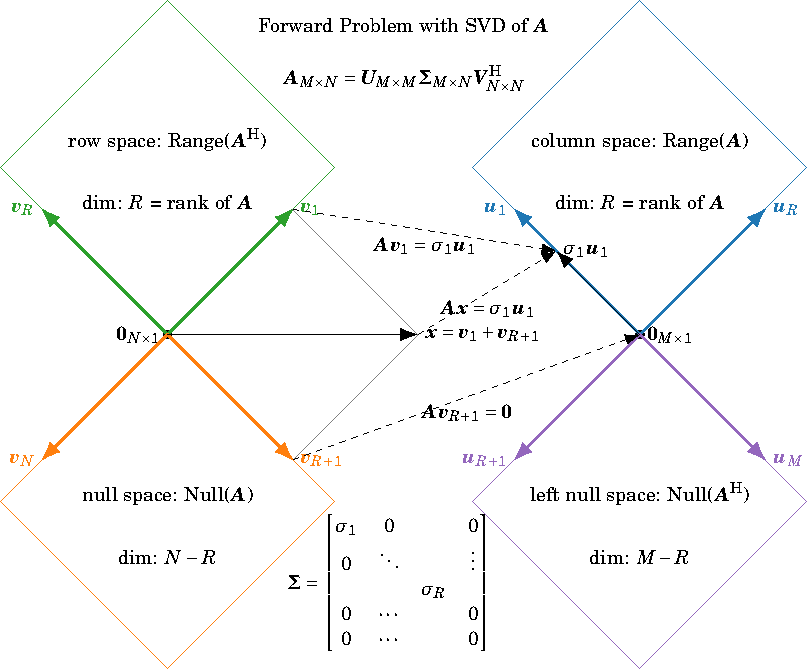
\includegraphics[width=0.79\textwidth]{../slides/four_subspaces.pdf}
\caption{The forward problem maps from row space to column space and from null space to zero vector.}
\label{fig:four_subspaces}
\end{subfigure}
\\
\begin{subfigure}[b]{1\textwidth}
\centering
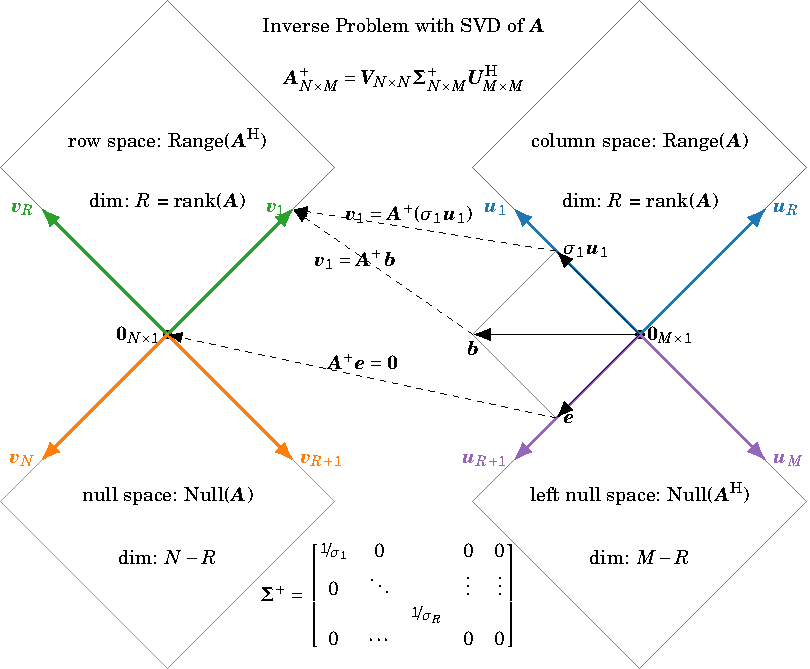
\includegraphics[width=0.79\textwidth]{../slides/pseudo_inverse_four_subspaces.pdf}
\caption{The inverse problem maps from column space to row space and from left null space to zero vector. The singular values are inverted. The pseudo-inverse of $\bm{A}$ is generally $\bm{A}^+ = \bm{V} \bm{\Sigma}^+ \bm{U}^\mathrm{H}$.}
\label{fig:pseudo_inverse_four_subspaces}
\end{subfigure}
\caption{
The four subspaces of a matrix encoded in the orthonormal SVD bases $\bm{V}$ (left, $\mathbb{R}^N$) and $\bm{U}$ (right, $\mathbb{R}^M$).
The forward (top) and the inverse (bottom) problem is schematically depicted with Gilbert Strang's 2D visualisation approach.
\\Special cases of pseudo-inverses are: the left-inverse for tall, thin, full column rank $\bm{A}$ (i.e. $M\gg N=R$), the right-inverse for wide, short, full row rank $\bm{A}$ (i.e. $N\gg M=R$) and the exact-inverse for square, full rank $\bm{A}$ (i.e. $M=N=R$).
}
\label{fig:SVD_subspaces}
\end{figure}

\section*{Exercise / Home Work Assignment}
Learning new things is about thoroughly thinking about the new things in our own style and pace.
Textbooks are a good choice to support this approach, as (older) textbooks have undergone profound quality checks, such that
we can assume the content to be valid and true.
Further, material that accompanies university lectures and tutorials is typically of very high quality and nearly error-free.
This way we shared research knowledge over centuries, probably with some success.
\\\\\noindent Learning new things is probably not about consuming too much AI generated content.

1. This content has---by the idea of statistics-driven text generation---no quality control,
such that we need to check validity on our own. But this can become rather tricky, if we just want to learn the new things, right?

2. Interaction with an AI is probably a nice and new way, but too much content and too fast interaction prevents us from really thinking about on our own.

3. Human interaction is probably even more efficient. Feel free to attend the lectures and tutorial in presence and ask many questions.
\\\\\noindent In this spirit and mindset, we could think about all of the above ideas and concepts for the three matrices
$$
\bm{A}_1 =
\begin{bmatrix}
4 & 0 & 4\\
2 & 0 & 2\\
4 & 2 & 6\\
4 & 4 & 8
\end{bmatrix}
\qquad
\bm{A}_2 =
\begin{bmatrix}
9 & 12 & 3 & 15\\
0 & 2 & 0 & 6\\
9 & 11 & 3 & 12
\end{bmatrix}
\qquad
\bm{A}_3 =
\begin{bmatrix}
3 & 0 & 0\\
0 & 0 & 2\\
0 & 1 & 0
\end{bmatrix}.
$$
While some results are comparably nice numbered scalars and vectors, many results are already too crazy for manual paper calculus.
%
Hence, it is highly recommended to implement all this in a small re-useable script or notebook using either Python/Numpy, Julia or Matlab. Using Julia in a Pluto notebook is very elegant for pure matrix algebra.
%
It is actually not about the specific numbers of the actual results, but about understanding the fundamentals behind these numbers.
%
The numbers in practical data are even more crazy and the problems are even more complicated, so we should manage to be very confident with this toy examples.
\\\\\noindent Again: With AI we might solve this task within seconds, but then neither the AI nor we have really understood, what is actually going on.
\textbf{Think for yourself}.
It might be a little pain in the beginning, but it is highly rewarding,
once the brain begins to process and understand. Consuming (a)social media will by far not compete with this special feeling of happiness.

\end{document}
